%------------------------------------------------------------------------------
% Author(s):
% Varaun Ramgoolie
%
% Copyright:
%  Copyright (C) 2020 Brad Bachu, Arjun Mohammed, Varaun Ramgoolie, Nicholas Sammy
%
%  This file is part of Applied-Mathematics-Unit2 and is distributed under the
%  terms of the MIT License. See the LICENSE file for details.
%
%  Description:
%     Year: 2008 June
%     Module: 3
%     Question: 5
%------------------------------------------------------------------------------

%------------------------------------------------------------------------------
% 5 a
%------------------------------------------------------------------------------

\begin{subquestions}

\subquestion

\begin{subsubquestions}
	
\subsubquestion

The Principle of Conservation of Energy states that, in a closed system, the total energy remains constant. The energy may change form but cannot be destroyed or created. \TODO{Find the best definition Brad!}

\subsubquestion

The Principle of Conservation of Linear Momentum states that, in a closed system, the total momentum of the system before a collision or explosion is equal to the total momentum of the system after the collision. 

\end{subsubquestions}

%------------------------------------------------------------------------------
% 5 b
%------------------------------------------------------------------------------

\begin{subsubquestions}
	
\subsubquestion

We are given a situation where a collision occurs and the bodies become coupled after the collision.

\textbf{\textit{Sketch and Translate:}} \\ \\
\begin{figure}[H]
	\begin{center}
		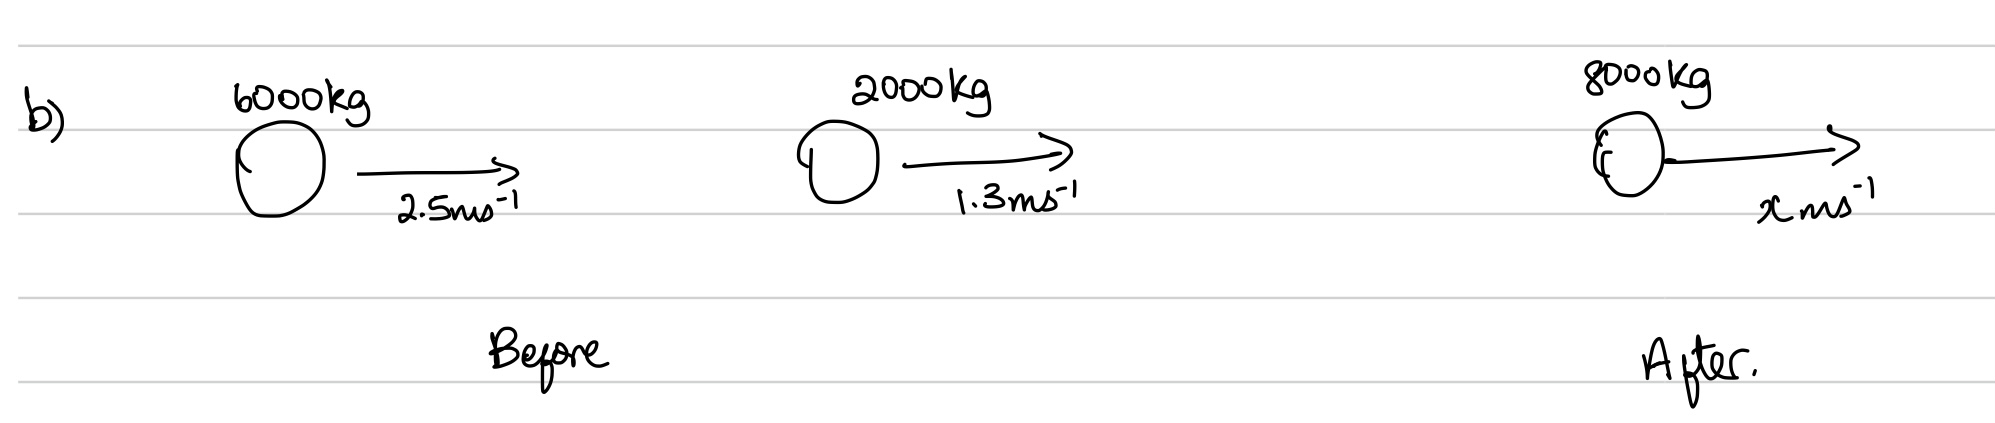
\includegraphics[scale=0.25]{../2008/figures/2008Jq5-1}
		\caption{\label{2008J:q5:Sketch1} Bodies colliding with each other.}
	\end{center}
\end{figure}	
We are asked to find the kinetic energy after the impact. 



\textbf{\textit{Simplify and Diagram:}} \\ \\ 
\TODO{define variables here!}
\begin{figure}[H]
	\begin{center}
		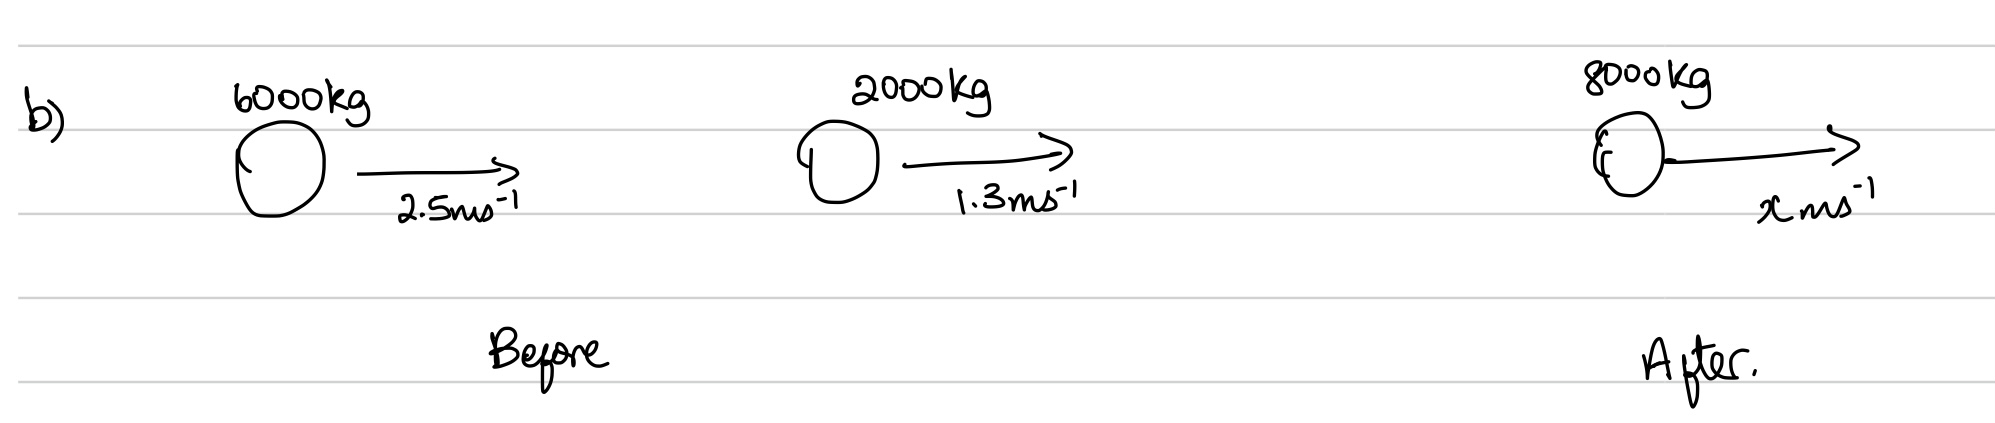
\includegraphics[scale=0.25]{../2008/figures/2008Jq5-1}
		\caption{\label{2008J:q5:Diagram1} Bodies colliding with each other.}
	\end{center}
\end{figure}	
We assume that the bodies act as point particles. We will also assume that the collision occurs in a closed system (no external forces acting on the system). We will take movement to the right as positive and we will assume that the bodies only move in 1 dimension. We can use the Law of Conservation of Momentum to solve this problem.
We will define the following:
\begin{itemize}
	\item $m_1$ is the mass of the 6000kg sphere, $m_1=6000$,
	\item $m_2$ is the mass of the 2000kg sphere, $m_2=2000$,
	\item $v_1$ is the velocity of the 6000kg sphere before collision, $v_1=2.5$,
	\item $v_2$ is the velocity of the 2000kg sphere before collision, $v_1=1.3$,
	\item $v_3$ is the velocity of the coupled body after collision.	
\end{itemize}



\textbf{\textit{Represent Mathematically:}} \\ \\
From the Law of Conservation of Momentum, we get that,
\begin{align}
	\text{Total Momentum Before collision} & = \text{Total Momentum After collision} \nn \\
	m_1v_1 + m_2v_2 & = (m_1+m_2)v_3 \,. \label{2008J:q5:VEqn1}
\end{align}

The kinetic energy of the coupled body after the collision can be given as,
\begin{align}
	KE = \frac{1}{2}(m_1+m_2)v_3^2 \,.
\end{align}


\textbf{\textit{Solve and Evaluate:}} \\ \\
From \req{2008J:q5:VEqn1}, we get,
\begin{align}
	m_1v_1 + m_2v_2 & = (m_1+m_2)v_3 \nn \\
	6000\times2.5 + 2000\times1.3 & = (6000+2000)v_3 \nn \\
	\implies v_3 & = \frac{15000+2600}{8000} \nn \\
	& = 2.2\text{ms}^{-1}
\end{align}

Therefore, we get that the kinetic energy after the collision is,
\begin{align}
	KE & = \frac{1}{2}(6000+2000)2.2^2 \nn \\
	   & = 19360J.
\end{align} 

%------------------------------------------------------------------------------

\subsubquestion

\textbf{\textit{Sketch and Translate:}} \\ \\
\{insert diagrams here\}
We can approach this question using Newton's Second Law. We will consider the 1000N force as the resultant force on the coupled body. The body will be brought to rest when the final velocity, $v$, is 0.




\textbf{\textit{Simplify and Diagram:}} \\ \\
We will assume that the coupled body moves only in 1 dimension. We will calculate the deceleration of the body by using Newton's Second Law, and then we can use our equations of motion to solve for the distance and time it takes to bring the body to rest. We will define the following as:
\begin{itemize}
	\item $m$ is the mass of the coupled body, $m-8000$,
	\item $u$ is the initial velocity of the coupled body, $u=v_3=2.2$,
	\item $v$ is the final velocity of the coupled body, $v=0$,
	\item $F$ is the braking force, $F=-1000N$,\footnote{This force has a negative sign as it is directed in the opposite direction to the coupled body's motion.}
	\item $a$ is the acceleration of the body,
	\item $s$ is the distance traveled by the body,
	\item $t$ is the time variable.
\end{itemize}



\textbf{\textit{Represent Mathematically:}} \\ \\ 
Using Newton's Second Law, we get that,
\begin{align}
	F & = ma \nn \\
	\implies a & = \frac{F}{m} \label{2008J:q5:AEqn1} \,.
\end{align}

To find the distance, we can use,
\begin{equation}
	v^2 = u^2 + 2as \label{2008J:q5:SEqn1} \,.
\end{equation}

To find the time, we can use,
\begin{equation}
	v = u+at \label{2008J:q5:TEqn1} \,.
\end{equation}




\textbf{\textit{Solve and Evaluate:}} \\ \\
Using \req{2008J:q5:AEqn1}, we get that,
\begin{align}
	a & = \frac{-1000}{8000} \nn \\
	  & = -0.125ms^{-2} \,. 
\end{align}

Using \req{2008J:q5:SEqn1}, we get that,
\begin{align}
	2.2^2 & = 0^2 + 2(-0.125)(s) \nn \\
	\implies s & = \frac{0^2-2.2^2}{2(-0.125)} \nn \\
	  & = 19.36m \,.
\end{align}

Using \req{2008J:q5:TEqn1}, we get that,
\begin{align}
	0 & = 2.2 - 0.125t \nn \\
	t & = \frac{0-2.2}{-0.125} \nn \\
	  & = 17.6s \,.
\end{align}

\end{subsubquestions}
	
\end{subquestions}